\documentclass[aspectratio=169,11pt]{beamer}

% -----------------------------------------------------------------------------
% Self-contained presentation setup
% -----------------------------------------------------------------------------
\usepackage[T1]{fontenc}
\usepackage{lmodern}
\usepackage{amsmath,amssymb,mathtools}
\usepackage{booktabs}
\usepackage{tabularx}
\usepackage{listings}
\usepackage{tikz}
\usepackage[most]{tcolorbox}
\usepackage{appendixnumberbeamer}
\usetikzlibrary{arrows.meta,calc,fit,matrix,positioning,shapes.geometric}

\usetheme{Boadilla}
\usecolortheme{seagull}
\setbeamertemplate{navigation symbols}{}
\setbeamertemplate{items}[circle]
\setbeamertemplate{enumerate items}[default]
\setbeameroption{hide notes}

\definecolor{osblue}{RGB}{28,86,145}
\definecolor{osgreen}{RGB}{36,125,91}
\definecolor{osorange}{RGB}{202,105,36}
\definecolor{osred}{RGB}{166,45,45}
\definecolor{osgray}{RGB}{74,85,104}
\setbeamercolor{structure}{fg=osblue}
\setbeamercolor{alerted text}{fg=osred}
\setbeamercolor{block title}{bg=osblue!15,fg=black}
\setbeamercolor{block body}{bg=osblue!4,fg=black}

\newcommand{\concept}[1]{\textcolor{osblue}{\textbf{#1}}}
\newcommand{\code}[1]{\texttt{#1}}
\newcommand{\smallnote}[1]{\par\vspace{0.2em}{\scriptsize\color{osgray}#1}}

\tcbset{
  enhanced,
  boxrule=.7pt,
  arc=1.5mm,
  left=1.2mm,right=1.2mm,top=.8mm,bottom=.8mm,
  colback=osblue!3,
  colframe=osblue!60
}

\lstset{
  basicstyle=\scriptsize\ttfamily,
  keywordstyle=\color{osblue}\bfseries,
  commentstyle=\color{osgreen!80!black},
  stringstyle=\color{osred},
  numbers=left,
  numberstyle=\tiny\color{osgray},
  numbersep=5pt,
  frame=single,
  rulecolor=\color{black!20},
  backgroundcolor=\color{black!2},
  breaklines=true,
  showstringspaces=false,
  columns=fullflexible,
  keepspaces=true
}

\setbeamertemplate{footline}{%
  \leavevmode%
  \hbox{%
    \begin{beamercolorbox}[wd=.18\paperwidth,ht=2.6ex,dp=1.1ex,center]{author in head/foot}
      \insertshortauthor
    \end{beamercolorbox}%
    \begin{beamercolorbox}[wd=.64\paperwidth,ht=2.6ex,dp=1.1ex,center]{title in head/foot}
      \insertshorttitle\ifx\insertsection\empty\else\enspace---\enspace\insertsection\fi
    \end{beamercolorbox}%
    \begin{beamercolorbox}[wd=.18\paperwidth,ht=2.6ex,dp=1.1ex,center]{date in head/foot}
      \insertframenumber{} / \inserttotalframenumber
    \end{beamercolorbox}%
  }
}

\AtBeginSection[]{
  \begin{frame}[plain,noframenumbering]{Road map}
    \tableofcontents[currentsection,hideothersubsections]
  \end{frame}
}

\title[Processes and Kernel State]{Process Abstraction, Kernel State, and Context Switching}
\subtitle{Week 3: Processes, threads, lifecycle, task records, and observation}
\author[SDB]{SDB}
\date{Autumn 2026}

\begin{document}

\begin{frame}[plain,noframenumbering]
  \titlepage
  \vspace{-1.2em}
  \begin{center}
    \small Intermediate/graduate engineering lecture set
  \end{center}
\end{frame}

\begin{frame}{Learning outcomes}
  By the end of this lecture set, you should be able to:
  \begin{enumerate}
    \item distinguish programs, processes, threads, address spaces, and kernel tasks;
    \item explain lifecycle transitions using runnable and blocked \emph{threads};
    \item identify process-wide versus thread-specific kernel state;
    \item trace \code{fork()}, \code{execve()}, exit, waiting, reparenting, and job control;
    \item describe the direct and microarchitectural costs of a context switch;
    \item reason about multicore placement, namespaces, cgroups, and resource accounting; and
    \item interpret Linux \code{/proc} and \code{ps} output without mistaking it for a literal PCB dump.
  \end{enumerate}
  \begin{tcolorbox}[title=Guiding question,colback=osorange!5,colframe=osorange!70]
    What state must the kernel preserve so that an execution can stop now and resume correctly later---possibly on another CPU?
  \end{tcolorbox}
\end{frame}

\begin{frame}{Road map}
  \tableofcontents
\end{frame}

% =============================================================================
\section{The Process Abstraction}
% =============================================================================

\begin{frame}{Program, process, and thread are different abstractions}
  \small
  \begin{tabularx}{\textwidth}{@{}lXX@{}}
    \toprule
    \textbf{Concept} & \textbf{Meaning} & \textbf{Representative state} \\
    \midrule
    Program & passive executable/data format stored or generated & instructions, metadata, interpreter request \\
    Process & protected resource and execution environment & address space, handles, credentials, namespaces \\
    Thread & schedulable instruction stream within a process & registers, stack, scheduling state, TLS \\
    Address space & virtual-memory translation/protection context & mappings, page tables, VM policies \\
    Kernel task & implementation-specific schedulable/managed entity & links to shared and per-thread records \\
    \bottomrule
  \end{tabularx}
  \begin{alertblock}{Most important correction}
    On mainstream general-purpose systems, the scheduler selects runnable \emph{threads/tasks}, not an indivisible process. A multithreaded process can have one thread running while another is blocked.
  \end{alertblock}
  \note{Introductory texts often use process states before introducing threads. Retain that model only as a single-threaded simplification. In Linux, a task is the schedulable entity, and sharing is controlled through clone relationships and shared objects.}
\end{frame}

\begin{frame}{A process is a bundle of shared resources}
  \begin{columns}[T,onlytextwidth]
    \column{0.48\textwidth}
      \centering
      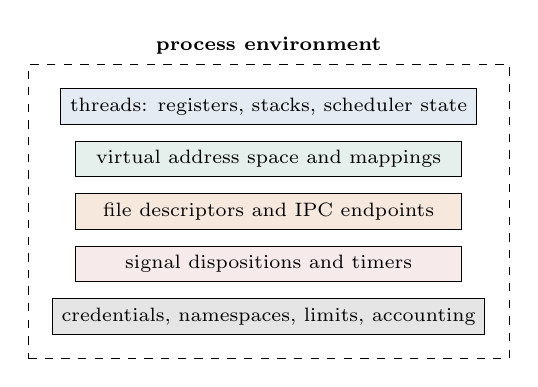
\begin{tikzpicture}[font=\scriptsize,node distance=2mm,every node/.style={align=center}]
        \node[draw,fill=osblue!12,minimum width=4.9cm] (t) {threads: registers, stacks, scheduler state};
        \node[draw,fill=osgreen!12,minimum width=4.9cm,below=of t] (vm) {virtual address space and mappings};
        \node[draw,fill=osorange!15,minimum width=4.9cm,below=of vm] (fd) {file descriptors and IPC endpoints};
        \node[draw,fill=osred!10,minimum width=4.9cm,below=of fd] (sig) {signal dispositions and timers};
        \node[draw,fill=black!10,minimum width=4.9cm,below=of sig] (sec) {credentials, namespaces, limits, accounting};
        \node[draw,dashed,fit=(t)(vm)(fd)(sig)(sec),inner sep=3mm,label=above:{\bfseries process environment}] {};
      \end{tikzpicture}
    \column{0.49\textwidth}
      \begin{itemize}
        \item The process abstraction supplies isolation, naming, accounting, and a unit for resource ownership.
        \item Threads deliberately share much process state, enabling low-cost communication but also shared failure fate.
        \item The kernel may distribute this state across many objects rather than store one monolithic PCB.
      \end{itemize}
      \begin{tcolorbox}[title=Design lens]
        Ask for each field: Is it per-thread, process-shared, reference-counted, inherited, copied, reset, or replaced?
      \end{tcolorbox}
  \end{columns}
\end{frame}

\begin{frame}{Identity is contextual, not one universal PID}
  \begin{columns}[T,onlytextwidth]
    \column{0.51\textwidth}
      Process-related identities can include:
      \begin{itemize}
        \item thread ID, process/thread-group ID, parent ID;
        \item process-group ID and session ID;
        \item real/effective/saved user and group IDs;
        \item namespace-relative PIDs;
        \item stable kernel handles such as Linux pidfds;
        \item security labels and audit identities.
      \end{itemize}
    \column{0.45\textwidth}
      \begin{alertblock}{PID reuse}
        A numeric PID is a temporary name. Between lookup and action, the original process can exit and the number can be reused. Handle-based interfaces reduce this race.
      \end{alertblock}
      \begin{tcolorbox}[title=Namespace consequence]
        The same task can have different PID values when viewed from nested PID namespaces.
      \end{tcolorbox}
  \end{columns}
  \note{Connect this slide to TOCTOU from Week 2. Opening /proc/PID files or using pidfd-based operations can reduce identity races, though exact guarantees vary by interface. Process groups and sessions are job-control identities, not scheduler groups.}
\end{frame}

\begin{frame}{Virtual address space: mappings, not a fixed four-segment box}
  \small
  \begin{columns}[T,onlytextwidth]
    \column{0.39\textwidth}
      \centering
      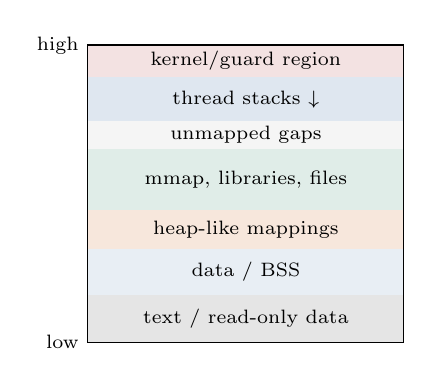
\begin{tikzpicture}[y=.47cm,font=\scriptsize]
        \draw[thick] (0,0) rectangle (4,8);
        \fill[osred!14] (0,7.15) rectangle (4,8); \node at (2,7.58) {kernel/guard region};
        \fill[osblue!14] (0,5.95) rectangle (4,7.15); \node at (2,6.55) {thread stacks $\downarrow$};
        \fill[black!4] (0,5.2) rectangle (4,5.95); \node at (2,5.58) {unmapped gaps};
        \fill[osgreen!14] (0,3.55) rectangle (4,5.2); \node at (2,4.38) {mmap, libraries, files};
        \fill[osorange!16] (0,2.5) rectangle (4,3.55); \node at (2,3.03) {heap-like mappings};
        \fill[osblue!10] (0,1.25) rectangle (4,2.5); \node at (2,1.88) {data / BSS};
        \fill[black!10] (0,0) rectangle (4,1.25); \node at (2,.63) {text / read-only data};
        \node[left] at (0,0) {low}; \node[left] at (0,8) {high};
      \end{tikzpicture}
    \column{0.57\textwidth}
      \begin{itemize}
        \item Virtual memory is sparse; regions are independent mappings with permissions and backing objects.
        \item Shared libraries, files, anonymous arenas, JIT code, shared memory, and multiple thread stacks complicate the textbook picture.
        \item ASLR changes placement; exact layout depends on architecture, ABI, loader, runtime, and security policy.
        \item Heap and stack growth directions are conventions, not defining properties of a process.
      \end{itemize}
      \begin{alertblock}{Address zero}
        Low virtual addresses are commonly left unmapped to catch null dereferences; user text does not generally begin at exactly zero.
      \end{alertblock}
  \end{columns}
  \note{Do not label the top region as always kernel-mapped: kernel page-table isolation and architecture choices differ. The diagram is conceptual. Also distinguish virtual size from resident physical memory; a mapping need not be resident.}
\end{frame}

\begin{frame}{Threads: shared state and private execution context}
  \small
  \begin{tabularx}{\textwidth}{@{}XX@{}}
    \toprule
    \textbf{Normally shared within a process} & \textbf{Normally per thread} \\
    \midrule
    virtual address space and code & general registers, PC, SP, flags \\
    heap/global memory mappings & user and kernel stack \\
    open-file table / many handles & scheduling class, priority, affinity \\
    current directory and many credentials & thread-local storage and robust-list state \\
    signal dispositions & signal mask and pending thread-directed signals \\
    resource limits and namespaces & CPU accounting and fault/debug state \\
    \bottomrule
  \end{tabularx}
  \begin{tcolorbox}[title=Consequence]
    Blocking one thread does not block its siblings unless they depend on the same lock, resource, or process-wide condition. One thread's memory corruption can damage every thread in the process.
  \end{tcolorbox}
\end{frame}

% =============================================================================
\section{Lifecycle, Creation, and Relationships}
% =============================================================================

\begin{frame}{Thread lifecycle: portable conceptual model}
  \centering
  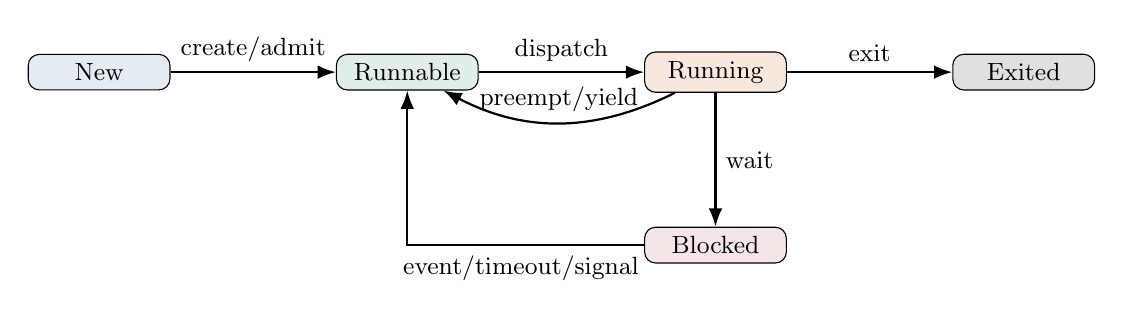
\begin{tikzpicture}[>=Latex,font=\small,node distance=1.7cm and 2.1cm,every node/.style={align=center}]
    \node[draw,rounded corners,fill=osblue!12,minimum width=1.8cm] (new) {New};
    \node[draw,rounded corners,fill=osgreen!14,minimum width=1.8cm,right=of new] (ready) {Runnable};
    \node[draw,rounded corners,fill=osorange!16,minimum width=1.8cm,right=of ready] (run) {Running};
    \node[draw,rounded corners,fill=osred!12,minimum width=1.8cm,below=of run] (block) {Blocked};
    \node[draw,rounded corners,fill=black!12,minimum width=1.8cm,right=of run] (term) {Exited};
    \draw[->,thick] (new)--node[above]{create/admit}(ready);
    \draw[->,thick] (ready)--node[above]{dispatch}(run);
    \draw[->,thick,bend left=27] (run) to node[above]{preempt/yield}(ready);
    \draw[->,thick] (run)--node[right]{wait}(block);
    \draw[->,thick] (block)-|node[pos=.26,below]{event/timeout/signal}(ready);
    \draw[->,thick] (run)--node[above]{exit}(term);
  \end{tikzpicture}
  \begin{itemize}
    \item \concept{Runnable} combines ``ready'' and currently executing; only one thread per logical CPU is running at an instant.
    \item \concept{Blocked} means an event is required before the thread can run; it is not simply waiting its turn for a CPU.
    \item Stop/tracing, uninterruptible sleep, parking, and zombie states are OS-specific refinements.
  \end{itemize}
  \note{The original deck allowed a ready process to be killed directly into a generic terminated state. Administrative termination is normally delivered through mechanisms that require kernel processing and may not complete instantly. Present this diagram as a logical scheduler model, not every internal state.}
\end{frame}

\begin{frame}{Linux task states do not map one-to-one to the textbook model}
  \small
  \begin{tabularx}{\textwidth}{@{}lXX@{}}
    \toprule
    \textbf{Code} & \textbf{Typical \code{ps} meaning} & \textbf{Interpretation} \\
    \midrule
    \code{R} & running or runnable & on a CPU or eligible for scheduling \\
    \code{S} & interruptible sleep & waiting; signals can wake/interrupt \\
    \code{D} & uninterruptible sleep & commonly waiting in a kernel path; not safely interruptible at that point \\
    \code{T/t} & stopped or traced & job-control stop or debugger/tracer stop \\
    \code{Z} & zombie & thread-group leader/process exit status awaits reaping \\
    \code{I} & idle kernel thread & kernel-specific idle state in some tools \\
    \bottomrule
  \end{tabularx}
  \begin{alertblock}{Snapshot caveat}
    State can change immediately after observation. Tools also aggregate or choose one thread's state; inspect per-thread data when diagnosing a multithreaded process.
  \end{alertblock}
\end{frame}

\begin{frame}{Creating a process image: \code{fork()} then \code{execve()}}
  \centering
  \resizebox{.94\textwidth}{!}{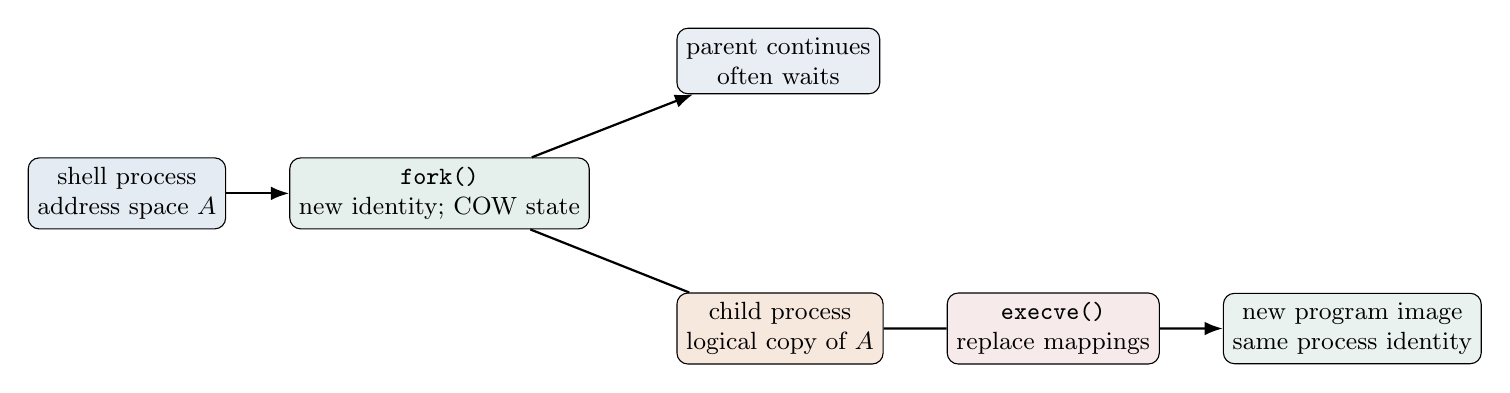
\begin{tikzpicture}[>=Latex,font=\small,node distance=8mm,every node/.style={align=center}]
    \node[draw,rounded corners,fill=osblue!12] (shell) {shell process\\address space $A$};
    \node[draw,rounded corners,fill=osgreen!12,right=of shell] (fork) {\code{fork()}\\new identity; COW state};
    \node[draw,rounded corners,fill=osblue!10,above right=8mm and 11mm of fork] (parent) {parent continues\\often waits};
    \node[draw,rounded corners,fill=osorange!15,below right=8mm and 11mm of fork] (child) {child process\\logical copy of $A$};
    \node[draw,rounded corners,fill=osred!10,right=of child] (exec) {\code{execve()}\\replace mappings};
    \node[draw,rounded corners,fill=osgreen!10,right=of exec] (prog) {new program image\\same process identity};
    \draw[->,thick] (shell)--(fork);
    \draw[->,thick] (fork)--(parent);
    \draw[->,thick] (fork)--(child)--(exec)--(prog);
  \end{tikzpicture}}
  \begin{itemize}
    \item \code{fork()} creates a child and returns in both parent and child; memory copy semantics are commonly implemented with copy-on-write.
    \item \code{execve()} does not create a new process. It replaces the calling process's program image and resets/preserves attributes according to a detailed contract.
  \end{itemize}
\end{frame}

\begin{frame}{Copy-on-write: semantics versus implementation}
  \begin{columns}[T,onlytextwidth]
    \column{0.49\textwidth}
      Immediately after \code{fork()}:
      \begin{itemize}
        \item parent/child PTEs reference shared frames;
        \item writable mappings become logically COW;
        \item page tables and metadata still require work;
        \item a write fault copies only the modified page.
      \end{itemize}
    \column{0.47\textwidth}
      \centering
      \resizebox{\linewidth}{!}{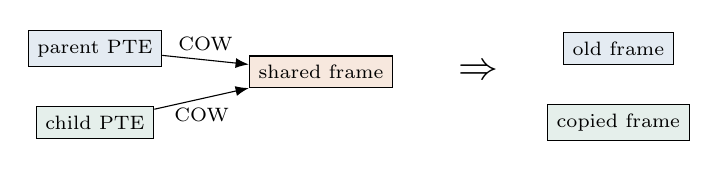
\begin{tikzpicture}[>=Latex,font=\scriptsize,node distance=5mm]
        \node[draw,fill=osblue!12] (p) {parent PTE};
        \node[draw,fill=osgreen!12,below=of p] (c) {child PTE};
        \node[draw,fill=osorange!15,right=1.1cm of p,yshift=-.3cm] (f) {shared frame};
        \draw[->] (p)--node[above]{COW}(f); \draw[->] (c)--node[below]{COW}(f);
        \node[right=7mm of f,font=\Large] (a) {$\Rightarrow$};
        \node[draw,fill=osblue!12,right=7mm of a,yshift=.3cm] (old) {old frame};
        \node[draw,fill=osgreen!12,below=of old] (copy) {copied frame};
      \end{tikzpicture}}
      \smallnote{Large processes can still pay for page-table duplication, reference accounting, TLB work, and later COW faults.}
  \end{columns}
  \note{Some systems provide alternatives such as posix_spawn or specialized clone/vfork-like mechanisms. Do not promise that COW makes fork cheap in every workload; pinned pages, huge mappings, many VMAs, and multithreaded runtime state matter.}
\end{frame}

\begin{frame}{What \code{execve()} replaces and what it preserves}
  \small
  \begin{tabularx}{\textwidth}{@{}XX@{}}
    \toprule
    \textbf{Replaced/reset examples} & \textbf{Preserved examples} \\
    \midrule
    user address-space mappings and code & PID and parent relationship \\
    thread set becomes one calling thread & many open descriptors unless close-on-exec \\
    caught signal dispositions reset to defaults & current directory and root directory \\
    alternate signal stack and many runtime objects & resource limits and selected credentials \\
    program arguments/environment are rebuilt & process group, session, controlling terminal \\
    architecture execution entry state & accounting/history defined by the OS \\
    \bottomrule
  \end{tabularx}
  \begin{alertblock}{Security-critical detail}
    Descriptor leakage across \code{execve()} can unintentionally grant the new program access to files, sockets, pipes, or privileged service endpoints. Prefer atomic close-on-exec creation flags.
  \end{alertblock}
  \smallnote{The exact contract includes exceptions for privilege transitions, tracing, secure execution, and OS-specific attributes; consult the platform specification.}
\end{frame}

\begin{frame}{Exit, zombie state, and reaping}
  \centering
  \resizebox{.92\textwidth}{!}{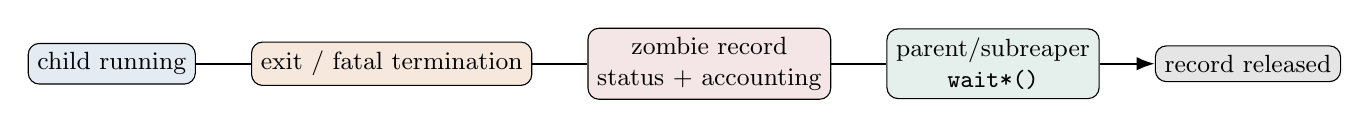
\begin{tikzpicture}[>=Latex,font=\small,node distance=7mm,every node/.style={align=center}]
    \node[draw,rounded corners,fill=osblue!12] (run) {child running};
    \node[draw,rounded corners,fill=osorange!15,right=of run] (exit) {exit / fatal termination};
    \node[draw,rounded corners,fill=osred!12,right=of exit] (z) {zombie record\\status + accounting};
    \node[draw,rounded corners,fill=osgreen!12,right=of z] (reap) {parent/subreaper\\\code{wait*()}};
    \node[draw,rounded corners,fill=black!10,right=of reap] (free) {record released};
    \draw[->,thick] (run)--(exit)--(z)--(reap)--(free);
  \end{tikzpicture}}
  \begin{itemize}
    \item Most execution resources are released at exit, but a small kernel record remains so an authorized waiter can collect status and usage.
    \item A zombie does not execute and does not retain its ordinary user address space.
    \item Persistent zombies indicate a parent/reaper bug and consume process-table/PID-related resources.
  \end{itemize}
  \note{Avoid saying the entire PCB remains. Linux retains the task identity and exit/accounting information needed for waiting, but much process state is already destroyed. In multithreaded processes, exit and wait semantics distinguish threads, thread groups, and children.}
\end{frame}

\begin{frame}{Orphans, subreapers, and PID namespaces}
  \small
  \begin{columns}[T,onlytextwidth]
    \column{0.52\textwidth}
      If a parent exits before a living child:
      \begin{itemize}
        \item the child continues unless another condition terminates it;
        \item it is reparented to an appropriate child subreaper or namespace init process;
        \item the new reaper becomes responsible for collecting its later exit status.
      \end{itemize}
      \begin{alertblock}{Correction}
        The new parent is not necessarily the host's PID 1 or \code{systemd}. Subreapers and nested PID namespaces alter the adoption path.
      \end{alertblock}
    \column{0.44\textwidth}
      \centering
      \resizebox{\linewidth}{!}{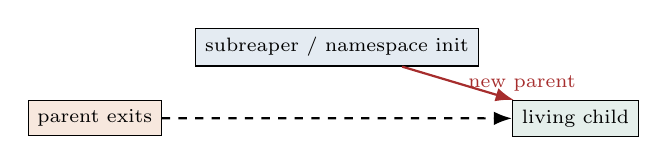
\begin{tikzpicture}[>=Latex,font=\scriptsize,node distance=6mm]
        \node[draw,fill=osblue!12] (sr) {subreaper / namespace init};
        \node[draw,fill=osorange!15,below left=of sr] (p) {parent exits};
        \node[draw,fill=osgreen!12,below right=of sr] (c) {living child};
        \draw[->,thick,dashed] (p)--(c);
        \draw[->,thick,osred] (sr)--node[right]{new parent}(c);
      \end{tikzpicture}}
      \smallnote{An orphan is not inherently erroneous; daemons and service supervisors intentionally manage parent/child lifecycles.}
  \end{columns}
\end{frame}

\begin{frame}{Process trees are not scheduling hierarchies}
  \begin{columns}[T,onlytextwidth]
    \column{0.46\textwidth}
      \centering
      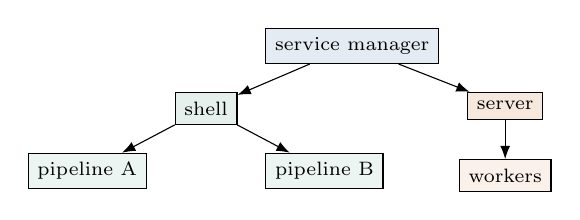
\begin{tikzpicture}[>=Latex,font=\scriptsize,node distance=5mm]
        \node[draw,fill=osblue!12] (init) {service manager};
        \node[draw,fill=osgreen!12,below left=of init] (shell) {shell};
        \node[draw,fill=osorange!15,below right=of init] (svc) {server};
        \node[draw,fill=osgreen!8,below left=of shell] (p1) {pipeline A};
        \node[draw,fill=osgreen!8,below right=of shell] (p2) {pipeline B};
        \node[draw,fill=osorange!9,below=of svc] (w) {workers};
        \draw[->] (init)--(shell); \draw[->] (init)--(svc);
        \draw[->] (shell)--(p1); \draw[->] (shell)--(p2); \draw[->] (svc)--(w);
      \end{tikzpicture}
    \column{0.50\textwidth}
      Parent/child relationships support creation, signals, waiting, and supervision. They do \emph{not} necessarily define:
      \begin{itemize}
        \item CPU-share allocation or scheduler groups;
        \item memory/resource-control hierarchy;
        \item security trust or ownership;
        \item terminal foreground/background membership.
      \end{itemize}
      \begin{tcolorbox}[title=Separate structures]
        cgroup trees, namespace relationships, process groups, sessions, and service-manager dependency graphs serve different purposes.
      \end{tcolorbox}
  \end{columns}
\end{frame}

\begin{frame}{Process groups, sessions, and terminal job control}
  \centering
  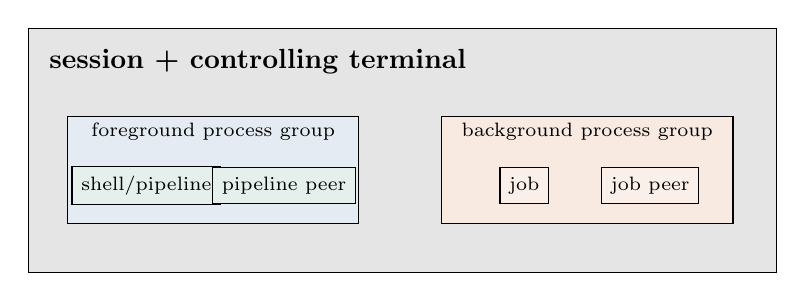
\begin{tikzpicture}[font=\scriptsize,node distance=4mm,every node/.style={align=center}]
    \node[draw,fill=black!10,minimum width=9.5cm,minimum height=3.1cm] (sess) {};
    \node[anchor=north west,font=\bfseries] at ($(sess.north west)+(.15,-.15)$) {session + controlling terminal};
    \node[draw,fill=osblue!12,minimum width=3.7cm,minimum height=1.35cm] at ($(sess.center)+(-2.4,-.25)$) (fg) {};
    \node at ($(fg.north)+(0,-.2)$) {foreground process group};
    \node[draw,fill=osgreen!12] at ($(fg.center)+(-.85,-.2)$) {shell/pipeline};
    \node[draw,fill=osgreen!12] at ($(fg.center)+(.9,-.2)$) {pipeline peer};
    \node[draw,fill=osorange!14,minimum width=3.7cm,minimum height=1.35cm] at ($(sess.center)+(2.35,-.25)$) (bg) {};
    \node at ($(bg.north)+(0,-.2)$) {background process group};
    \node[draw,fill=osorange!10] at ($(bg.center)+(-.8,-.2)$) {job};
    \node[draw,fill=osorange!10] at ($(bg.center)+(.8,-.2)$) {job peer};
  \end{tikzpicture}
  \begin{itemize}
    \item The terminal driver directs generated job-control signals to the foreground process group.
    \item Background execution means shell/job-control status, not independence from all terminal effects or parent relationships.
    \item \code{Ctrl-Z}, \code{fg}, and \code{bg} manipulate stopped jobs and process groups, not individual scheduler states alone.
  \end{itemize}
\end{frame}

% =============================================================================
\section{Kernel Records and Scheduling State}
% =============================================================================

\begin{frame}{There is rarely one literal ``PCB'' structure}
  \begin{columns}[T,onlytextwidth]
    \column{0.52\textwidth}
      \concept{PCB} is a useful conceptual name for kernel-maintained state needed to manage a process. Production kernels commonly decompose it into:
      \begin{itemize}
        \item per-thread scheduling and saved execution state;
        \item shared memory-management objects;
        \item file/handle tables and filesystem context;
        \item credentials, namespaces, signals, timers;
        \item parent/child and process-group relationships;
        \item accounting, tracing, security, and resource-control links.
      \end{itemize}
    \column{0.44\textwidth}
      \begin{alertblock}{Why decomposition?}
        Sharing, copy-on-write, independent lifetime, cache locality, locking discipline, and feature evolution all favor referenced objects over one giant record.
      \end{alertblock}
      \begin{tcolorbox}[title=Terminology]
        Use ``task/thread control block'' for schedulable state and ``process-wide state'' for shared resources when precision matters.
      \end{tcolorbox}
  \end{columns}
  \note{The term PCB is pedagogical and architecture-neutral. Linux task_struct is not simply the PCB for a process: each thread has a task_struct and many fields point to shared objects such as mm_struct, files_struct, signal_struct, and credentials.}
\end{frame}

\begin{frame}{Conceptual kernel object graph}
  \centering
  \resizebox{.95\textwidth}{!}{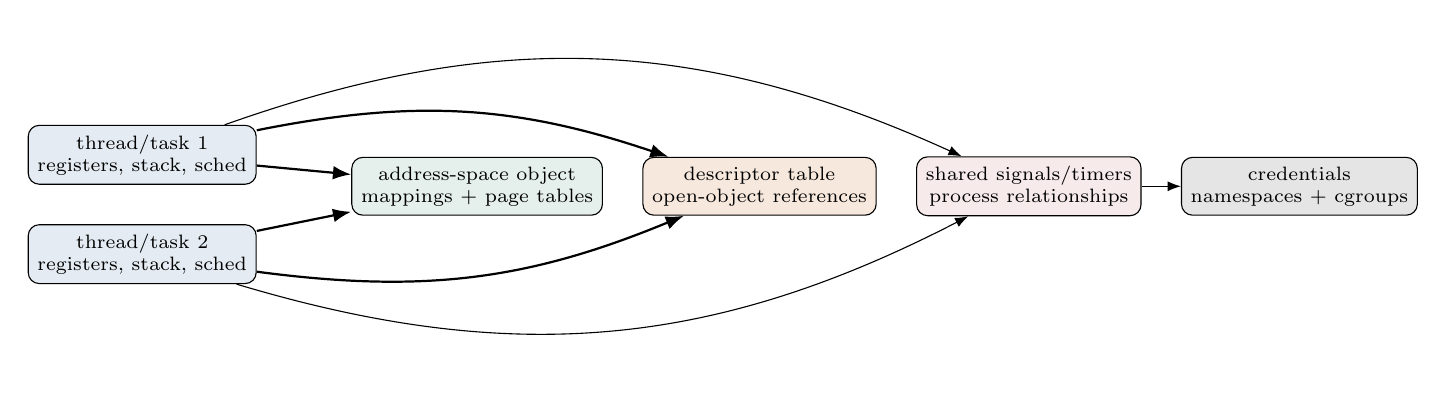
\begin{tikzpicture}[>=Latex,font=\scriptsize,node distance=5mm,every node/.style={align=center}]
    \node[draw,rounded corners,fill=osblue!12] (t1) {thread/task 1\\registers, stack, sched};
    \node[draw,rounded corners,fill=osblue!12,below=of t1] (t2) {thread/task 2\\registers, stack, sched};
    \node[draw,rounded corners,fill=osgreen!12,right=1.2cm of t1,yshift=-.4cm] (mm) {address-space object\\mappings + page tables};
    \node[draw,rounded corners,fill=osorange!15,right=of mm] (files) {descriptor table\\open-object references};
    \node[draw,rounded corners,fill=osred!10,right=of files] (sig) {shared signals/timers\\process relationships};
    \node[draw,rounded corners,fill=black!10,right=of sig] (sec) {credentials\\namespaces + cgroups};
    \draw[->,thick] (t1)--(mm); \draw[->,thick] (t2)--(mm);
    \draw[->,thick] (t1) to[bend left=15] (files); \draw[->,thick] (t2) to[bend right=15] (files);
    \draw[->] (t1) to[bend left=22] (sig); \draw[->] (t2) to[bend right=22] (sig);
    \draw[->] (sig)--(sec);
  \end{tikzpicture}}
  \begin{itemize}
    \item Reference counts and locks coordinate shared lifetime and concurrency.
    \item \code{fork}/\code{clone} semantics determine which objects are copied, shared, or newly allocated.
    \item Exit can release some objects immediately while retaining identity/accounting for waiting.
  \end{itemize}
\end{frame}

\begin{frame}{What must be saved for a context switch?}
  \begin{columns}[T,onlytextwidth]
    \column{0.49\textwidth}
      \textbf{Architectural/thread state}
      \begin{itemize}
        \item program counter, stack pointer, flags;
        \item callee/architecture-required registers;
        \item floating-point/vector state as required;
        \item debug, TLS, control, and security state;
        \item kernel stack location and return path.
      \end{itemize}
    \column{0.48\textwidth}
      \textbf{Execution environment}
      \begin{itemize}
        \item address-space/page-table context when it changes;
        \item CPU-local scheduler/current-task pointer;
        \item accounting, tracing, and lock/preemption state;
        \item architecture mitigations and lazy/eager state policies.
      \end{itemize}
  \end{columns}
  \begin{tcolorbox}[title=Important nuance]
    A switch between threads in one process may preserve the address space. A switch between processes may use ASID/PCID-tagged translations rather than flushing the entire TLB.
  \end{tcolorbox}
\end{frame}

\begin{frame}{Context-switch timeline}
  \centering
  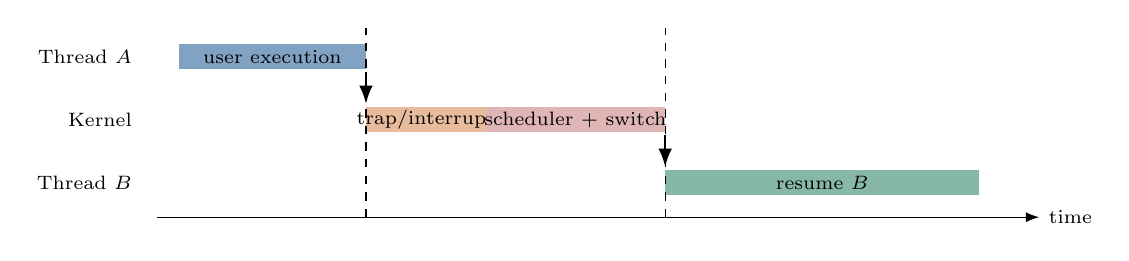
\begin{tikzpicture}[x=.95cm,y=.8cm,font=\scriptsize,>=Latex]
    \node[anchor=east] at (0,3) {Thread $A$};
    \node[anchor=east] at (0,2) {Kernel};
    \node[anchor=east] at (0,1) {Thread $B$};
    \draw[->] (.2,.45)--(12,.45) node[right]{time};
    \fill[osblue!55] (.5,2.8) rectangle (3.0,3.2); \node at (1.75,3) {user execution};
    \fill[osorange!45] (3.0,1.8) rectangle (4.6,2.2); \node at (3.8,2) {trap/interrupt};
    \fill[osred!35] (4.6,1.8) rectangle (7.0,2.2); \node at (5.8,2) {scheduler + switch};
    \fill[osgreen!55] (7.0,.8) rectangle (11.2,1.2); \node at (9.1,1) {resume $B$};
    \draw[dashed] (3,.45)--(3,3.45); \draw[dashed] (7,.45)--(7,3.45);
    \draw[->,thick] (3,2.75)--(3,2.25);
    \draw[->,thick] (7,1.75)--(7,1.25);
  \end{tikzpicture}
  \begin{enumerate}
    \item An interrupt, exception, syscall, block, or explicit yield enters the kernel.
    \item The current thread's necessary state is preserved; scheduler policy may select another runnable thread.
    \item Low-level code changes task/stack/address-space context and returns into the selected thread.
  \end{enumerate}
  \note{A timer interrupt does not force a different thread if policy keeps the current one. Likewise, a syscall is not a context switch unless a different task is selected. The boundary between interrupt handling, scheduler code, and low-level switch code is implementation-specific.}
\end{frame}

\begin{frame}{Context-switch cost is direct plus indirect}
  \begin{columns}[T,onlytextwidth]
    \column{0.49\textwidth}
      \textbf{Direct latency}
      \begin{itemize}
        \item entry/exit and scheduler execution;
        \item saving/restoring register state;
        \item run-queue locking/accounting;
        \item address-space or mitigation work.
      \end{itemize}
    \column{0.47\textwidth}
      \textbf{Indirect latency}
      \begin{itemize}
        \item cold/private cache lines;
        \item TLB and page-walk effects;
        \item branch predictor/prefetch disruption;
        \item NUMA/cache migration cost;
        \item contention induced by extra concurrency.
      \end{itemize}
  \end{columns}
  \begin{alertblock}{Measurement discipline}
    There is no universal context-switch time. Specify architecture, kernel, mitigation/configuration, thread relationship, CPU migration, cache state, workload, and metric.
  \end{alertblock}
\end{frame}

\begin{frame}{Run queues and wait queues serve different questions}
  \small
  \begin{columns}[T,onlytextwidth]
    \column{0.48\textwidth}
      \centering
      \resizebox{\linewidth}{!}{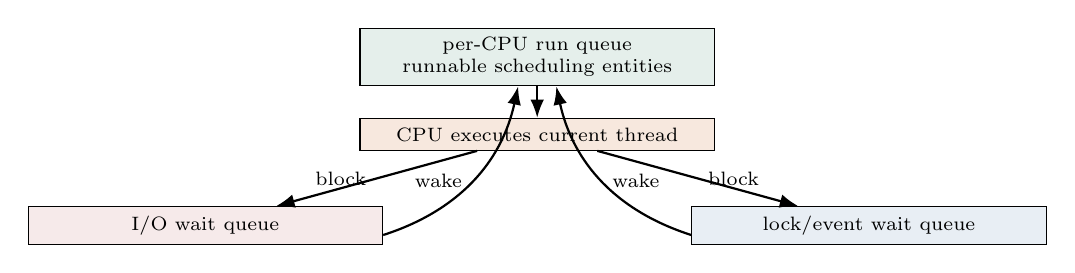
\begin{tikzpicture}[>=Latex,font=\scriptsize,node distance=4mm,every node/.style={align=center}]
        \node[draw,fill=osgreen!12,minimum width=4.5cm] (rq) {per-CPU run queue\\runnable scheduling entities};
        \node[draw,fill=osorange!15,minimum width=4.5cm,below=of rq] (cpu) {CPU executes current thread};
        \node[draw,fill=osred!10,minimum width=4.5cm,below left=7mm and -3mm of cpu] (io) {I/O wait queue};
        \node[draw,fill=osblue!10,minimum width=4.5cm,below right=7mm and -3mm of cpu] (lock) {lock/event wait queue};
        \draw[->,thick] (rq)--(cpu);
        \draw[->,thick] (cpu)--node[left]{block}(io);
        \draw[->,thick] (cpu)--node[right]{block}(lock);
        \draw[->,thick,bend right=30] (io) to node[left]{wake}(rq);
        \draw[->,thick,bend left=30] (lock) to node[right]{wake}(rq);
      \end{tikzpicture}}
    \column{0.49\textwidth}
      \begin{itemize}
        \item A run queue answers: \emph{which runnable task should this CPU execute?}
        \item A wait queue links sleepers to the event or condition that can make them runnable.
        \item Modern kernels use multiple scheduler-class data structures, per-CPU queues, load balancing, timers, and wakeup placement.
        \item ``Job queue'' is a historical batch abstraction, not a universal production-kernel structure.
      \end{itemize}
  \end{columns}
\end{frame}

\begin{frame}{Intrusive queues and task lifetime}
  \begin{columns}[T,onlytextwidth]
    \column{0.52\textwidth}
      A task record may contain embedded linkage for several structures:
      \begin{itemize}
        \item scheduler/run-queue nodes;
        \item parent/child and sibling lists;
        \item wait queues and timers;
        \item process-group/session membership;
        \item tracing, cgroup, and namespace indexes.
      \end{itemize}
      \begin{tcolorbox}[title=Why intrusive structures?]
        They avoid separate allocation and support constant-time linkage, but require strict invariants: one link field cannot simultaneously belong to incompatible lists.
      \end{tcolorbox}
    \column{0.44\textwidth}
      \begin{alertblock}{Concurrency challenge}
        Task lookup, exit, wakeup, migration, and observation race across CPUs. Kernels combine locks, reference counts, RCU-like techniques, and carefully ordered state transitions.
      \end{alertblock}
      \smallnote{A task can disappear while another subsystem is trying to inspect it; stable references matter.}
  \end{columns}
\end{frame}

% =============================================================================
\section{Multicore Placement and Resource Control}
% =============================================================================

\begin{frame}{Multicore scheduling: placement is part of process performance}
  \small
  \begin{columns}[T,onlytextwidth]
    \column{0.47\textwidth}
      \centering
      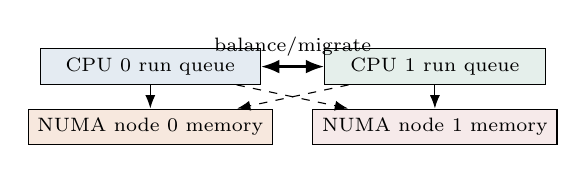
\begin{tikzpicture}[>=Latex,font=\scriptsize,node distance=3mm]
        \node[draw,fill=osblue!12,minimum width=2.8cm] (c0) {CPU 0 run queue};
        \node[draw,fill=osgreen!12,minimum width=2.8cm,right=8mm of c0] (c1) {CPU 1 run queue};
        \node[draw,fill=osorange!15,minimum width=2.8cm,below=of c0] (n0) {NUMA node 0 memory};
        \node[draw,fill=osred!10,minimum width=2.8cm,below=of c1] (n1) {NUMA node 1 memory};
        \draw[<->,thick] (c0)--node[above]{balance/migrate}(c1);
        \draw[->] (c0)--(n0); \draw[->] (c1)--(n1);
        \draw[->,dashed] (c0)--(n1); \draw[->,dashed] (c1)--(n0);
      \end{tikzpicture}
    \column{0.50\textwidth}
      \begin{itemize}
        \item Per-CPU run queues reduce global contention but require load balancing.
        \item Affinity can preserve cache/NUMA locality; excessive pinning can create imbalance.
        \item Wakeup placement considers idle CPUs, cache history, topology, energy, and policy.
        \item Simultaneous multithreading shares execution resources even when logical CPUs are distinct.
      \end{itemize}
      \begin{alertblock}{Migration cost}
        Moving a runnable thread is cheap in bookkeeping terms but can be expensive through lost cache locality and remote-memory access.
      \end{alertblock}
  \end{columns}
\end{frame}

\begin{frame}{Resource limits, accounting, and cgroups}
  \small
  \begin{tabularx}{\textwidth}{@{}lXX@{}}
    \toprule
    \textbf{Mechanism} & \textbf{Scope} & \textbf{Purpose} \\
    \midrule
    per-process limits & inherited soft/hard limits & cap descriptors, memory, CPU time, process creation \\
    credentials/capabilities & task/process security context & authorize operations and reduce privilege \\
    accounting & per-thread/process/group counters & usage reporting, billing, diagnosis, policy feedback \\
    cgroups & hierarchical groups of tasks & CPU share/quota, memory pressure, I/O control, process counts \\
    affinity/cpusets & allowed CPU and memory nodes & placement, isolation, NUMA policy \\
    service-manager policy & supervised unit/container & restart, dependency, lifetime, environment \\
    \bottomrule
  \end{tabularx}
  \begin{tcolorbox}[title=Hierarchy distinction]
    A cgroup hierarchy is independent of the parent/child process tree. A service can regroup descendants, and unrelated processes can share one resource-control group.
  \end{tcolorbox}
\end{frame}

\begin{frame}{Namespaces virtualize a process's view}
  \begin{columns}[T,onlytextwidth]
    \column{0.51\textwidth}
      Linux namespaces can isolate views of:
      \begin{itemize}
        \item process IDs and parent relationships;
        \item mounts/filesystem namespace;
        \item networking interfaces/routes/ports;
        \item users and capability interpretation;
        \item IPC objects, hostname, and time domains.
      \end{itemize}
    \column{0.45\textwidth}
      \begin{tcolorbox}[title=Container connection]
        A container is a set of ordinary processes constrained by namespaces, cgroups, credentials, filesystem setup, and security policy. It is not a special process state.
      \end{tcolorbox}
      \begin{alertblock}{Shared kernel}
        Namespace isolation changes visibility and naming; it does not create a separate kernel or eliminate shared-kernel attack surfaces.
      \end{alertblock}
  \end{columns}
\end{frame}

\begin{frame}{Signals, cancellation, and process-wide effects}
  \begin{itemize}
    \item Signals can be process-directed or thread-directed; delivery selects an eligible thread under platform rules.
    \item Each thread has a signal mask, while many dispositions are process-shared.
    \item Stop, continue, termination, and core-dump actions can affect the entire thread group.
    \item A blocked syscall may return \code{EINTR}, be transparently restarted, or complete partially depending on the call and signal configuration.
    \item Graceful process termination is a protocol: stop accepting work, cancel/wake threads, release resources, and report status.
  \end{itemize}
  \begin{alertblock}{Asynchrony}
    State observed before sending a signal may already be stale; signal delivery and handler execution are not instantaneous transaction boundaries.
  \end{alertblock}
\end{frame}

% =============================================================================
\section{Observing Processes on Linux}
% =============================================================================

\begin{frame}{\code{/proc} is a generated interface, not a PCB memory dump}
  \begin{columns}[T,onlytextwidth]
    \column{0.52\textwidth}
      procfs exposes kernel-generated views such as:
      \begin{itemize}
        \item \code{/proc/PID/status}: identity, state, memory summaries, capabilities;
        \item \code{/proc/PID/stat}: compact counters/state for tools;
        \item \code{/proc/PID/maps}: virtual-memory mappings;
        \item \code{/proc/PID/fd}: descriptor symlinks;
        \item \code{/proc/PID/task/TID}: per-thread views;
        \item \code{/proc/PID/ns} and \code{cgroup}: isolation/resource context.
      \end{itemize}
    \column{0.44\textwidth}
      \begin{alertblock}{Three caveats}
        \begin{enumerate}
          \item Fields are formatted projections, not raw structures.
          \item Separate reads need not form one atomic snapshot.
          \item Permission, namespaces, hidepid policy, and process exit can limit or race access.
        \end{enumerate}
      \end{alertblock}
      \begin{tcolorbox}[title=Thread inspection]
        For scheduling diagnosis, inspect \code{/proc/PID/task/TID} rather than assuming one process-wide state.
      \end{tcolorbox}
  \end{columns}
  \note{Correct the original claim that status directly maps to the PCB. VmRSS is an estimate/snapshot with kernel-specific accounting semantics, and fields evolve. procfs is Linux-specific; other Unix-like systems expose different interfaces.}
\end{frame}

\begin{frame}[fragile]{A practical observation workflow}
\begin{lstlisting}[language=bash]
ps -eLo pid,tid,ppid,pgid,sid,psr,stat,ni,comm --sort=pid,tid
cat /proc/$$/status
cat /proc/$$/sched
ls -l /proc/$$/fd
sed -n '1,20p' /proc/$$/maps
grep -E 'State|Pid|Tgid|Threads|Cpus_allowed_list' /proc/$$/status
\end{lstlisting}
  \begin{columns}[T,onlytextwidth]
    \column{0.48\textwidth}
      Ask:
      \begin{itemize}
        \item Which TIDs share a TGID?
        \item Which CPU last ran each thread?
        \item Which mappings and descriptors are shared?
      \end{itemize}
    \column{0.48\textwidth}
      Do not conclude:
      \begin{itemize}
        \item \code{R} means continuously consuming a CPU;
        \item a counter explains causality;
        \item one sample represents steady behavior.
      \end{itemize}
  \end{columns}
\end{frame}

\begin{frame}{Interpreting common \code{/proc/PID/status} fields}
  \small
  \begin{tabularx}{\textwidth}{@{}lXX@{}}
    \toprule
    \textbf{Field} & \textbf{Meaning} & \textbf{Caution} \\
    \midrule
    \code{Pid/Tgid/PPid} & thread/process-group/parent identities & namespace-relative and reusable \\
    \code{State} & current task state summary & instantaneous and per task \\
    \code{Threads} & number of threads in the thread group & can change concurrently \\
    \code{VmSize} & virtual address-space size summary & not physical memory consumption \\
    \code{VmRSS} & resident-set estimate/summary & shared pages and accounting complicate attribution \\
    \code{Cpus\_allowed\_list} & permitted logical CPUs & permission is not current placement \\
    context-switch counters & voluntary/involuntary classifications & definitions are kernel-specific; no causal trace \\
    \code{Cap*}/\code{Uid}/\code{Gid} & credentials/capability masks & interpret in namespace/security context \\
    \bottomrule
  \end{tabularx}
\end{frame}

\begin{frame}{Memory views: \code{maps}, RSS, PSS, and working set}
  \begin{columns}[T,onlytextwidth]
    \column{0.49\textwidth}
      \begin{itemize}
        \item \code{maps}: address ranges, permissions, offsets, and backing names.
        \item RSS: resident pages mapped by a process, including shared pages.
        \item PSS: shared-page cost divided among mapping processes.
        \item USS/private pages: pages uniquely attributable under a tool's definition.
        \item Working set: pages actively needed over a time window; not one static procfs counter.
      \end{itemize}
    \column{0.47\textwidth}
      \begin{alertblock}{Attribution problem}
        Shared libraries, page cache, copy-on-write, deduplication, huge pages, and kernel memory make ``memory used by one process'' policy-dependent.
      \end{alertblock}
      \begin{tcolorbox}[title=Diagnosis]
        Pair mappings with faults, reclaim, pressure-stall information, and time-series behavior rather than relying on one RSS sample.
      \end{tcolorbox}
  \end{columns}
\end{frame}

\begin{frame}{Counters versus traces}
  \begin{columns}[T,onlytextwidth]
    \column{0.48\textwidth}
      \textbf{Counters answer ``how much?''}
      \begin{itemize}
        \item CPU time, faults, switches, I/O bytes;
        \item low overhead and aggregatable;
        \item weak causal ordering.
      \end{itemize}
    \column{0.48\textwidth}
      \textbf{Traces answer ``what happened when?''}
      \begin{itemize}
        \item wakeup, block, migration, syscall events;
        \item supports latency decomposition;
        \item greater volume and perturbation risk.
      \end{itemize}
  \end{columns}
  \begin{tcolorbox}[title=Tool matching]
    Use \code{ps}/procfs for snapshots, \code{pidstat}/\code{perf stat} for rates and counters, and scheduler/eBPF/perf traces for wakeup-to-run latency and causality.
  \end{tcolorbox}
\end{frame}

% =============================================================================
\section{Synthesis}
% =============================================================================

\begin{frame}{End-to-end example: a server thread handles a request}
  \centering
  \resizebox{.96\textwidth}{!}{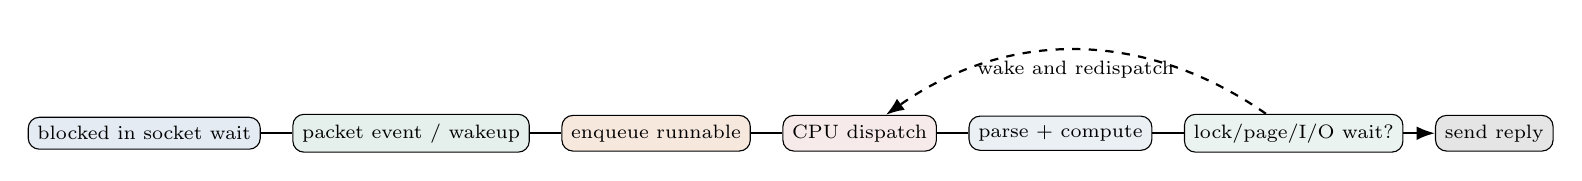
\begin{tikzpicture}[>=Latex,font=\scriptsize,node distance=4mm,every node/.style={align=center}]
    \node[draw,rounded corners,fill=osblue!12] (sleep) {blocked in socket wait};
    \node[draw,rounded corners,fill=osgreen!12,right=of sleep] (irq) {packet event / wakeup};
    \node[draw,rounded corners,fill=osorange!15,right=of irq] (rq) {enqueue runnable};
    \node[draw,rounded corners,fill=osred!10,right=of rq] (sched) {CPU dispatch};
    \node[draw,rounded corners,fill=osblue!9,right=of sched] (run) {parse + compute};
    \node[draw,rounded corners,fill=osgreen!9,right=of run] (block) {lock/page/I/O wait?};
    \node[draw,rounded corners,fill=black!10,right=of block] (reply) {send reply};
    \draw[->,thick] (sleep)--(irq)--(rq)--(sched)--(run)--(block)--(reply);
    \draw[->,thick,dashed,bend right=35] (block) to node[below]{wake and redispatch}(sched);
  \end{tikzpicture}}
  \begin{itemize}
    \item Kernel task state records lifecycle; shared process objects supply memory, descriptors, and credentials.
    \item Scheduler queues and wakeup placement determine runnable delay; locks, faults, and devices create blocked intervals.
    \item A process-level average can hide one pathological worker thread or CPU migration pattern.
  \end{itemize}
\end{frame}

\begin{frame}{Misconceptions corrected}
  \small
  \begin{tabularx}{\textwidth}{@{}X@{\quad$\Rightarrow$\quad}X@{}}
    \toprule
    \textbf{Misconception} & \textbf{Precise statement} \\
    \midrule
    The scheduler runs processes. & It normally schedules threads/tasks; process is a resource boundary. \\
    Ready means loaded in main memory. & Runnable means eligible for a CPU; paging/residency is a separate concern. \\
    One PCB contains everything. & Kernels decompose per-thread and shared state across referenced objects. \\
    Context switch saves every register every time. & Saved state depends on ABI, architecture, path, and lazy/eager policy. \\
    A zombie still owns its full memory. & Most resources are gone; exit/accounting identity remains for reaping. \\
    Every orphan is adopted by host PID 1. & Subreapers and PID namespaces determine the reparenting target. \\
    Background means detached from the terminal. & It means not in the foreground process group; terminal/session links may remain. \\
    \code{/proc/PID/status} is the PCB. & It is a formatted, partial, racing projection of kernel state. \\
    \bottomrule
  \end{tabularx}
\end{frame}

\begin{frame}{Key takeaways}
  \begin{itemize}
    \item A process is a protected, shared execution environment; threads are the schedulable instruction streams.
    \item Creation and execution are distinct: \code{fork()} creates identity/state, while \code{execve()} replaces the program image.
    \item Kernel process state is an object graph with independent lifetimes, sharing rules, and synchronization.
    \item Context switching includes direct kernel work and indirect cache/TLB/NUMA costs.
    \item Parent trees, process groups, namespaces, and cgroups are separate relationship structures.
    \item Observation is sampling: correlate per-thread snapshots, counters, and traces before drawing causal conclusions.
  \end{itemize}
  \begin{tcolorbox}[title=Transfer question,colback=osgreen!5,colframe=osgreen!65]
    When a task blocks, ask: what condition makes it runnable, which queue records the wait, who performs the wakeup, where will it run, and what shared state must remain valid?
  \end{tcolorbox}
\end{frame}

\begin{frame}{Laboratory: follow a process through its lifecycle}
  \begin{enumerate}
    \item Write a parent that starts two children, redirects one pipe, and reaps both with \code{waitpid()}.
    \item Observe PID, PPID, PGID, SID, TID, state, CPU, and descriptors using \code{ps} and procfs.
    \item Stop/continue one process and record state changes.
    \item Deliberately delay reaping to observe a zombie, then reap it.
    \item Trace scheduling/wakeup events and explain runnable versus blocked time.
    \item Repeat inside a PID namespace/container and compare visible identities.
  \end{enumerate}
  \begin{alertblock}{Safety}
    Use only processes you own. Do not alter system-wide \code{/proc/sys} settings for this laboratory.
  \end{alertblock}
\end{frame}

\begin{frame}{Next week: CPU scheduling}
  \begin{itemize}
    \item objectives: response time, turnaround, fairness, throughput, deadlines;
    \item FCFS, SJF/SRTF, round robin, priorities, and feedback queues;
    \item starvation, aging, priority inversion, and bounded blocking;
    \item multicore load balancing, affinity, topology, and energy;
    \item quantitative schedule construction and metric calculation.
  \end{itemize}
  \begin{tcolorbox}[title=Preparation]
    Create a timeline for three jobs with different arrival and service times. Compute response, waiting, and turnaround under FCFS and round robin.
  \end{tcolorbox}
\end{frame}

% =============================================================================
\appendix
\section{Appendix}
% =============================================================================

\begin{frame}{Knowledge check: abstraction and lifecycle}
  \begin{enumerate}
    \item Can two threads of one process simultaneously be in \code{R} and \code{S} states?
    \item Which process attributes survive \code{execve()}, and why is close-on-exec important?
    \item Why can a large \code{fork()} be expensive even if the child immediately executes another program?
    \item What information remains for a zombie, and what has already been released?
    \item Why can a PID-based kill script target the wrong process?
    \item Distinguish parent/child, process-group, cgroup, and namespace relationships.
  \end{enumerate}
  \note{Answers: (1) yes, states are per thread. (2) identity and selected resource context/descriptors survive by contract; leaked descriptors transfer authority. (3) page tables, VM metadata, references, TLB work. (4) exit status/accounting/identity remain; ordinary execution and most resources are gone. (5) PID reuse and races. (6) lifecycle, job control, resource hierarchy, and view/isolation respectively.}
\end{frame}

\begin{frame}{Knowledge check: switching and queues}
  \begin{enumerate}
    \item Does every timer interrupt cause a context switch to another thread?
    \item When can switching between threads avoid an address-space change?
    \item Give three indirect costs not captured by timing low-level switch code.
    \item What event moves a blocked task to a run queue?
    \item Why are per-CPU run queues scalable, and what new problem do they create?
    \item Why is one context-switch counter insufficient to diagnose latency?
  \end{enumerate}
\end{frame}

\begin{frame}[fragile]{Robust child creation and reaping skeleton}
\begin{lstlisting}[language=C]
pid_t pid = fork();
if (pid < 0) fail("fork");
if (pid == 0) {
    execlp("worker", "worker", (char *)NULL);
    static const char msg[] = "exec failed\n";
    (void)write(STDERR_FILENO, msg, sizeof msg - 1);
    _exit(127);
}

int status;
while (waitpid(pid, &status, 0) < 0) {
    if (errno != EINTR) fail("waitpid");
}
if (WIFEXITED(status)) report_exit(WEXITSTATUS(status));
else if (WIFSIGNALED(status)) report_signal(WTERMSIG(status));
\end{lstlisting}
  \smallnote{A production supervisor must also define descriptor inheritance, signal masks, process groups, timeouts, cancellation, and what to do if the parent crashes.}
\end{frame}

\begin{frame}{Exercise: classify state ownership}
  For each item, classify it as usually per-thread, process-shared, separately reference-counted, or policy-dependent:
  \begin{enumerate}
    \item program counter and user stack;
    \item virtual-memory mapping table;
    \item file descriptor and open-file description;
    \item signal disposition and signal mask;
    \item CPU affinity and cgroup membership;
    \item credentials and namespace membership;
    \item parent relationship and process group;
  \end{enumerate}
  \begin{tcolorbox}[title=Extension]
    For \code{fork()}, \code{pthread\_create()}, and \code{execve()}, state whether each item is copied, shared, reset, preserved, or replaced.
  \end{tcolorbox}
\end{frame}

\begin{frame}{Exercise: diagnose a stalled service}
  Symptoms: low CPU utilization, high request latency, several threads in \code{D}, and rising involuntary context-switch counts.
  \begin{enumerate}
    \item List at least four competing hypotheses.
    \item Which per-thread procfs fields and counters would you sample?
    \item Which trace events establish wakeup-to-run versus device-wait latency?
    \item How could CPU affinity or NUMA placement contribute?
    \item Why does a high context-switch count not prove context switches are the root cause?
  \end{enumerate}
\end{frame}

\begin{frame}{Exercise: compute direct switch overhead}
  Suppose a workload runs for a full $8\,\mathrm{ms}$ quantum and incurs one measured direct switch cost of $6\,\mu\mathrm{s}$ at each handoff.
  \begin{enumerate}
    \item Estimate the direct overhead fraction:
      \[
        \frac{6\,\mu\mathrm{s}}{8\,\mathrm{ms}+6\,\mu\mathrm{s}}.
      \]
    \item Repeat for a $200\,\mu\mathrm{s}$ quantum.
    \item Explain why neither number estimates cache, TLB, migration, queueing, or lock effects.
    \item Give a workload in which a shorter quantum improves user-visible latency despite higher overhead.
  \end{enumerate}
  \note{The numerical results are about 0.075 percent and 2.91 percent. The denominator convention should be stated; alternate definitions may divide by useful time alone. Use the exercise to separate direct mechanism cost from policy consequences.}
\end{frame}

\begin{frame}{Further study}
  \begin{itemize}
    \item Linux task model: task structures, shared objects, clone flags, pidfds.
    \item Scheduling internals: run queues, wakeup placement, scheduler classes.
    \item Process supervision: subreapers, service managers, process groups, signals.
    \item Resource isolation: cgroups, namespaces, pressure-stall information.
    \item Observability: scheduler tracing, eBPF, perf, off-CPU analysis.
    \item Assurance: task-lifetime races, RCU, reference counting, formal state machines.
  \end{itemize}
  \begin{center}
    \Large Questions?
  \end{center}
\end{frame}

\end{document}

